\documentclass[xcolor={svgnames},
  %hyperref={colorlinks,citecolor=Blue,linkcolor=Blue,urlcolor=DarkBlue}, 
  hyperref={colorlinks}, 
  spanish, 12pt]{beamer}
  \mode<presentation>
  
  \usefonttheme[onlymath]{serif}
  \setbeamertemplate{theorems}[ams style] 
  
  
\usetheme{metropolis}
 \useinnertheme{rectangles} 
\setbeamertemplate{navigation symbols}{}
%\setbeamertemplate{caption}[numbered]
%\useoutertheme{infolines}
\usepackage{cleveref}

\setbeamercovered{highly dynamic}

\newcounter{saveenumi}
\newcommand{\seti}{\setcounter{saveenumi}{\value{enumi}}}
\newcommand{\conti}{\setcounter{enumi}{\value{saveenumi}}}

\resetcounteronoverlays{saveenumi}

%\usepackage{beamerthemebars}
\usepackage{fontenc}
\usepackage{graphicx}
\usepackage[utf8]{inputenc}
\usepackage[spanish,mexico]{babel}
\usepackage{fontenc}
\usepackage{amsmath}
\usepackage{amsthm}
\usepackage{amssymb}
\usepackage{graphicx}
\usepackage{mathrsfs}
\usepackage{yfonts}
%\usepackage{hyperref}
\usepackage{enumerate}
\usepackage{mathtools}
\usepackage{textcomp}
\usepackage{lmodern}
\usepackage{fancyvrb}
\usepackage{multicol}
\usepackage{color}

\DefineVerbatimEnvironment{ColorVerbatim}{Verbatim}%
  {formatcom=\color{purple},commandchars=\\\{\}}
  
\usepackage{etoolbox}

\BeforeBeginEnvironment{Verbatim}{\begingroup\color{purple}}%
\AfterEndEnvironment{Verbatim}{\endgroup}%
%\usepackage{etoolbox}
% \AtBeginEnvironment{enumerate}{\begin{multicols}{2}}    %%% this line
% \AtEndEnvironment{enumerate}{\end{multicols}}            %%% and this one
% \usepackage{multicol}
%\usepackage[usenames,dvipsnames,svgnames,table]{xcolor}
%\usepackage[urlcolor=blue]{hyperref}
%\numberwithin{section}{part}
\numberwithin{equation}{section} %% Comment out for sequentially-numbered
\numberwithin{figure}{section} %% Comment out for sequentially-numbered

% Automatically generate section title slides in beamer?
% Add support for \subsubsectionpage
\def\subsubsectionname{\translate{}}
\def\insertsubsubsectionnumber{\arabic{subsubsection}}
\setbeamertemplate{subsubsection page}
{
  \begin{centering}
    {\usebeamerfont{subsubsection name}\usebeamercolor[fg]{subsubsection name}\subsubsectionname}%~\insertsubsubsectionnumber}
    \vskip1em\par
    \begin{beamercolorbox}[sep=4pt,center]{part title}
      \usebeamerfont{subsubsection title}\insertsubsubsection\par
    \end{beamercolorbox}
  \end{centering}
}
\def\subsubsectionpage{\usebeamertemplate*{subsubsection page}}

\AtBeginSection{\frame{\sectionpage}}
\AtBeginSubsection{\frame{\subsectionpage}}
\AtBeginSubsubsection{\frame{\subsubsectionpage}}

\theoremstyle{plain}
  \newtheorem{thm}{Teorema}[section]
  \newtheorem{prop}{Proposici\'on}[section]
  \newtheorem{lem}[thm]{Lema}
  \newtheorem{cor}[thm]{Corolario}
  %\newtheorem{rem}{Observaci\'on}[chapter]
  \newtheorem*{sol}{Soluci\'on}
  \newtheorem{alg}{Algoritmo}[section]
  \newtheorem{solved}{Ejercicio Resuelto}
  \newtheorem{evc}{Evaluaci\'on Continua}

\theoremstyle{definition}
  \newtheorem{defn}{Definici\'on}[section]
  \newtheorem{conj}{Conjectura}[section]
  \newtheorem{exmp}{Ejemplo}[section]
  \newtheorem{exe}{Evaluaci\'on Continua}[section]
  \newtheorem{prob}{Problema}[section]
  \newtheorem{rem}{Observaci\'on}[section]
  \newtheorem*{ax}{Axioma}
  \newtheorem{tdv}{Tabla de Verdad}

\theoremstyle{remark}
  \newtheorem{claim}{Afirmaci\'on}[section]
  %\newtheorem{rem}{Observaci\'on}[chapter]
  %\newtheorem*{note}{Nota}
  \newtheorem{case}{Caso}
  \newtheorem{hint}{Sugerencia}[section]


\numberwithin{equation}{section}
\newcommand{\p}{\partial}
%\newcommand{\T}{\mathbb{T}}
\newcommand{\R}{\mathbb{R}}
\newcommand{\N}{\mathbb{N}}
\newcommand{\Q}{\mathbb{Q}}
\newcommand{\abs}[1]{\left|#1\right|}
\newcommand{\f}{\phi}
\newcommand{\vphi}{\varphi}
\newcommand{\vf}{\varphi}
\newcommand{\flow}[2]{\varphi^{#1}\left( #2 \right)}
\renewcommand{\d}[1]{\dot{#1}}
\renewcommand{\r}{\rho}
\newcommand{\A}{\mathcal{A}}
\newcommand{\gam}{\gamma}
\newcommand{\lam}{\lambda}
\renewcommand{\a}{\alpha}
\renewcommand{\b}{\beta}
\newcommand{\om}{\omega}
\newcommand{\iso}{\simeq}
\newcommand{\tensor}{\otimes}
\newcommand{\Z}{\mathbb{Z}}
\newcommand{\set}[1]{\left\{ #1 \right\}}
\newcommand{\inc}{\hookrightarrow}
\renewcommand{\L}{\mathcal{L}}
\renewcommand{\H}{\mathcal{H}}
\newcommand{\D}{\mathcal{D}}
\newcommand{\converge}[1]{\xrightarrow{#1}}
\renewcommand{\cot}{T^{*}}
\newcommand{\cott}[1]{T^{*}\T^{#1}}
\newcommand{\ep}{\epsilon}
\newcommand{\inp}[1]{\langle #1 \rangle}
%\newcommand{\G}{\mathcal{G}}
\newcommand{\hu}{\textbf{h}}
\newcommand{\deck}[1]{\operatorname{Dake}\left( #1 \right)}
\newcommand{\til}[1]{\tilde{#1}}
\newcommand{\Gam}{\Gamma}
\newcommand{\grad}{\nabla}
\newcommand{\del}{\delta}
\newcommand{\id}{\operatorname{Id}}
\newcommand{\Del}{\Delta}
\newcommand{\var}{\Delta}
\newcommand{\avch}[2]{\frac{\Delta #1}{\Delta #2}}
\newcommand{\Avch}[2]{\dfrac{\Delta #1}{\Delta #2}}
\newcommand{\Err}{\operatorname{Err}}
\newcommand{\imply}{\rightarrow}
\newcommand{\wed}{\wedge}
\newcommand{\biconditional}{\longleftrightarrow}
\newcommand{\yields}{\vdash}
\newcommand{\onlyif}{\Rightarrow}
\newcommand{\uset}{\mathbb{U}}
\newcommand{\minus}{\backslash}
\newcommand{\symdif}{\oplus}
\newcommand{\rel}[1]{\boxed{{\color{blue}\textbf{#1}}}}
\newcommand{\dom}[1]{\operatorname{Dom}\left( #1 \right)}
\newcommand{\im}[1]{\operatorname{Im}\left( #1 \right)}
\newcommand{\nrel}[1]{\boxed{{\color{red}\not}{\color{orange}\textbf{#1}}}}
\newcommand{\comp}[2]{#1 \circ #2}

%\date{\today}
\title{Matem\'aticas Discretas\\
L\'ogica y C\'alculo Proposicional}
\author[Juliho Castillo]{\href{https://www.youtube.com/channel/UCb1i-EtybaWWX5urFfmMUWQ}{M. en C. Juliho Castillo}}

\institute[ITESM CCM]{Tec de Monterrey, Campus Ciudad de M\'exico}
\date{\today}

\begin{document}

\logo{
 
\includegraphics[width=3cm,keepaspectratio=true]{./logo.png}
 %LOGO-CECYTEO.png: 200x200 pixel, 72dpi, 7.06x7.06 cm, bb=0 0 200 200
}

\frame{
\titlepage
}

\frame{\tableofcontents}

% \AtBeginSubsection[]
% {
%   \begin{frame}
%     \tableofcontents[currentsubsection]
%   \end{frame}
% }

\section{L\'ogica y C\'alculo Proposicional}

\begin{frame}
    Muchos algoritmos y demostraciones usan expresiones l\'ogicas tales como
    \texttt{si p entonces q}. Entonces es necesario conocer los casos en los cuales esas expresiones son \texttt{ciertas} o \texttt{falsas}. Discutiremos esto en esta unidad. 
\end{frame}



\begin{frame}
    Tambi\'en investigamos el valor de verdad de enunciados cuantificados, que son aquellos que usan los cuantificadores l\'ogicos \texttt{para todo...} y \texttt{existe...}
\end{frame}

\subsection{Proposiciones y Declaraciones Compuestas}

\begin{frame}
    Una proposici\'on es un enunciado declarativo que puede ser cierto o falso, pero no ambos. 
\end{frame}

\begin{frame}
    \begin{exmp}
        ?`Cu\'al de los siguientes enunciados es una proposici\'on?
        \begin{multicols}{2}
            \begin{enumerate}
                \item El hielo flota en el agua.
                \item China est\'a en Europa.
                \item $2+2=4$
                \item $2+2=5$
                \item ?`A donde vas?
                \item Haz tu tarea.
            \end{enumerate}
        \end{multicols}
    \end{exmp}
    
\end{frame}

\subsubsection{Proposiciones compuestas}

\begin{frame}
    Muchas proposiciones est\'an \texttt{compuestas} de proposiciones m\'as simples, llamadas \emph{subproposiciones}, por medio de \emph{conectores l\'ogicos.} \pause Una proposici\'on se dice que es \emph{primitiva} si no puede descomponerse en proposiciones m\'as simples.
\end{frame}

\begin{frame}
    Por ejemplo, las siguientes proposiciones son compuestas
    \begin{itemize}
        \item ``Las rosas son rojas y las violetas son azules''
        \item ``Juan es inteligente y estud\'ia hasta muy noche''
    \end{itemize}
    
\end{frame}

\begin{frame}
    La propiedad fundamental de una proposici\'on compuesta es que su valor de verdad est\'a completamente deteminado por los valores de verdad de sus subproposiciones y la manera en la cual est\'an conectadas para formar la proposici\'on compuesta. 
\end{frame}

\subsection{Operaciones L\'ogicas B\'asicas}

\begin{frame}
    En esta secci\'on discutiremos las tres operaciones l\'ogical b\'asicas: conjunci\'on , disjunci\'on  y la negaci\'on.
\end{frame}

\subsubsection{Conjunci\'on $p \wed q$}

\begin{frame}
    Cualesquiera dos proposiciones $p,q$ pueden ser combinadas por la palabra ``y'' para formar una proposici\'on compuesta llamada \emph{conjunci\'on} que se escribe $p\wed q.$
\end{frame}

\begin{frame}
    \begin{defn}
        Si tanto $p$ como $q$ son ciertas, entonces $p \wed q$ es cierta; en otro caso $p\wed q$ es falsa.
    \end{defn}
    
\end{frame}

\begin{frame}
    \begin{rem}
        Para entender mejor como se conectan los valores de verdad, generalmente se utilizan \emph{tablas de verdad.} \pause 
        
        Por brevedad $1$ representar\'a el valor \texttt{cierto}, mientras que $0$ representar\'a \texttt{falso}
    \end{rem}
    
\end{frame}

\begin{frame}
    \begin{tdv}[Conjunci\'on]
        \label{tdv:and}
        \begin{center}
            \begin{tabular}{|l|l|l|}\hline
                $p$ & $q$ & $p \wed q$\\\hline
                1 & 1 & 1\\\hline
                1 & 0 & 0\\\hline
                0 & 1 & 0\\\hline
                0 & 0 & 0\\\hline
            \end{tabular}
        \end{center}
        
    \end{tdv}
    
\end{frame}

\begin{frame}
    En este curso, usaremos el \emph{sistema algebr\'aico de computo} \texttt{SageMath}, el cu\'al est\'a escrito con base en el lenguaje de programaci\'on \texttt{Python} e incorpora diversos paquetes de \texttt{OpenSource}.
    \pause
    
    Puede acceder a este sistema, a trav\'es de \href{https://cloud.sagemath.com/}{https://cloud.sagemath.com/} 
    
\end{frame}

\begin{frame}
    Construimos la tabla de verdad de la conjunci\'on en el siguiente scritp \href{https://cloud.sagemath.com/projects/12787063-cafe-4f3b-a2e0-905f8b83cf3b/files/MD01_TRDV01_AND.sagews}{https://goo.gl/hEF5os}
    \begin{center}
        \includegraphics[height=5cm,keepaspectratio=true]{../MD_SMC/MD01_TDV01_AND.png}
        % MD01_TDV01_AND.png: 0x0 pixel, 300dpi, 0.00x0.00 cm, bb=
    \end{center}
    
\end{frame}

\begin{frame}
    \begin{exmp}
        ?`Cu\'al de las siguientes proposiciones es cierta?
        
        \begin{enumerate}
            \item El hielo flota y $2+2=4$
            \item El hielo flota y $2+2=5$
            \item China est\'a en Europa y $2+2=4$
            \item China est\'a en Europa y $2+2=5$
        \end{enumerate}
        
    \end{exmp}
    
\end{frame}

\subsubsection{Disjunci\'on $p \vee q$}

\begin{frame}
    Cualesquiera dos proposiciones $p,q$ pueden ser combinadas por la palabra ``o'' para formar una proposici\'on compuesta llamada \emph{disjunci\'on} que se escribe $p \vee q .$
\end{frame}

\begin{frame}
    \begin{defn}
        Si tanto $p$ como $q$ son falsas, entonces $p \vee q$ es falsa; en otro caso $p\vee q$ es verdadera.
    \end{defn}
    
\end{frame}


\begin{frame}
    \begin{tdv}[Disjunci\'on]
        \label{tdv:or}
        \begin{center}
            \begin{tabular}{|l|l|l|}\hline
                $p$ & $q$ & $p \vee q$\\\hline
                1 & 1 & 1\\\hline
                1 & 0 & 1\\\hline
                0 & 1 & 1\\\hline
                0 & 0 & 0\\\hline
            \end{tabular}
        \end{center}
        
    \end{tdv}
    
\end{frame}

\begin{frame}
    Construimos la tabla de verdad de la disjunci\'on en el siguiente scritp \href{https://cloud.sagemath.com/projects/12787063-cafe-4f3b-a2e0-905f8b83cf3b/files/MD01_TDV02_OR.sagews}{https://goo.gl/5kXzNI}
    \begin{center}
        \includegraphics[height=5cm,keepaspectratio=true]{../MD_SMC/MD01_TDV02_OR.png}
        % MD01_TDV01_AND.png: 0x0 pixel, 300dpi, 0.00x0.00 cm, bb=
    \end{center}
    
\end{frame}

\begin{frame}
 \begin{rem}
  Algunas veces \texttt{``p o q''} se entiende en el sentido exclusivo: Puede ocurrir \texttt{p} o \texttt{q}, \emph{pero no ambos,} que es diferente a la definici\'on anterior. Sin embargo, existe un conector llamado de hecho \texttt{o exclusivo,} que cumple esta definici\'on y consideraremos m\'as adelante. 
 \end{rem}

\end{frame}

\subsubsection{Negaci\'on $\neg p$}

\begin{frame}
 Dada cualquier proposici\'on $p,$ otra proposici\'on llamada \emph{negaci\'on} de $p$ puede ser formada escribien \emph{``No es cierto que...''} o \emph{``Es falso que...''} antes de \texttt{p}.
 \pause
 De manera m\'as sencilla, decimos \texttt{no $p$} y escribimos $\neg p.$
\end{frame}

\begin{frame}
 
\begin{defn}[Negaci\'on]
 Si $p$ es cierta, entonces $\neg p$ es falsa; pero si $p$ es falsa, $\neg p$ es cierta.
\end{defn}

\end{frame}

\begin{frame}
    \begin{tdv}[Negaci\'on]
        \label{tdv:not}
        \begin{center}
            \begin{tabular}{|l|l|}\hline
                $p$ & $\neg p$\\\hline
                1 & 0 \\\hline
                0 & 1 \\\hline
            \end{tabular}
        \end{center}
        
    \end{tdv}
    
\end{frame}

\begin{frame}
    Construimos la tabla de verdad de la disjunci\'on en el siguiente scritp \href{https://cloud.sagemath.com/projects/12787063-cafe-4f3b-a2e0-905f8b83cf3b/files/MD01_TDV03_NOT.sagews}{https://goo.gl/sgCfkC}
    \begin{center}
        \includegraphics[height=5cm,keepaspectratio=true]{../MD_SMC/MD01_TDV03_NOT.png}
        % MD01_TDV01_AND.png: 0x0 pixel, 300dpi, 0.00x0.00 cm, bb=
    \end{center}
    
\end{frame}

\subsection{Proposiciones y Tablas de Verdad}

\begin{frame}
 Sea $P(p,q,...)$ una expresi\'on construida con variables l\'ogicas $p,q,...,$ que toman valores de \texttt{verdadero ``V''} o \texttt{falso ``F''}, a trav\'es de conectores l\'ogicos como $\wed, \, \vee, \, \neg$ y otros  que discutiremos m\'as adelante.
 \pause
 
 Tales expresiones $P(p,q,...)$ son llamadas \emph{proposiciones.}
\end{frame}

\begin{frame}
 La propiedad principal de una proposici\'on $P(p,q,...)$ es que sus valores de verdad s\'olo dependen del valor de sus varibles. 
 \pause
 
 Una manera simple y concisa de mostrar esta relaci\'on es a trav\'es de una \emph{tabla de verdad.}
\end{frame}

\begin{frame}
 \begin{exmp}
  Contruir la tabla de verdad de la proposici\'on
  $$\neg \left( p \wed \neg q \right).$$
 \end{exmp}

\end{frame}

\begin{frame}
 Construimos la tabla de verdad de la proposici\'on anterior con el siguiente script \href{https://goo.gl/V2Axzi}{https://goo.gl/V2Axzi}
\begin{center}
        \includegraphics[height=5cm,keepaspectratio=true]{../MD_SMC/MD01_TDV04.png}
        % MD01_TDV01_AND.png: 0x0 pixel, 300dpi, 0.00x0.00 cm, bb=
\end{center}
 
\end{frame}

\begin{frame}
 \begin{tdv}[$\neg\left( p \wed \neg q \right)$] 
  \begin{tabular}{lllll}
p & q & not q & p and not q & not( p and not q) \\
$1$ & $1$ & $0$ & $0$ & $1$ \\
$1$ & $0$ & $1$ & $1$ & $0$ \\
$0$ & $1$ & $0$ & $0$ & $1$ \\
$0$ & $0$ & $1$ & $0$ & $1$ \\
\end{tabular}
 \end{tdv}

\end{frame}

\begin{frame}
 \begin{rem}
  Para evitar el uso excesivo de parentesis, algunas veces adoptamos una jerarqu\'ia para los conectores l\'ogicos. 
  \pause
  
  De manera especifica $\neg$ tiene prioridad sobre $\wed,$ que a su vez tiene prioridad sobre $\vee$.
 \end{rem}
\end{frame}

\begin{frame}
 Por ejemplo, $$\neg p \wed q$$ significa $$\left( \neg p \right) \wed q$$ \pause y no
 $$
 \neg(p \wed q).
 $$
\end{frame}

\begin{frame}
 \frametitle{M\'etodo alternativo de construir una tabla de verdad}
\begin{center}
\begin{tabular}{|l|l|l|l|l|l|l|}\hline
 $p$ & $q$ & $\neg$ & $(p$ & $\wed$ & $\neg$ & q) \\\hline
 $1$ & $1$ &  &  & &  & \\\hline
 $1$ & $0$ &  &  & &  & \\\hline
 $0$ & $1$ &  &  & &  & \\\hline
 $0$ & $0$ &  &  & &  & \\\hline
\end{tabular}
\end{center}

\end{frame}

\begin{frame}
\begin{evc} Construya las tablas de verdad de las siguientes proposiciones
\begin{enumerate}
 \item $p\vee \neg p$
 \item $p\wed \neg p$
 \item $\neg\left( p \vee q \right)$
 \item $\neg p \wed \neg q$
 \item $\neg\left( p \wed q \right)$
 \item $\neg p \vee \neg q$
\end{enumerate}


\end{evc}

\end{frame}


\subsection{Tautolog\'ias y Contradicciones}

\begin{frame}
 Algunas proposiciones $P(p,q,...)$ son siempre ciertas, no importa los valores de verdad de las variables $p,q,...$ 
 \pause 
 
 Tales proposiciones se conocen como \emph{tautolog\'ias.}
\end{frame}

\begin{frame}
 De manera similar, algunas proposiciones $P(p,q,...)$ son siempre falsas, no importa los valores de verdad de las variables $p,q,...$ 
 \pause 
 
 Tales proposiciones se conocen como \emph{contradicciones.}
\end{frame}

\begin{frame}
 \begin{exmp}
  Construya las tablas de verdad de $p \wed \neg p$ y $p \vee \neg p.$
 \end{exmp}

\end{frame}

\subsection{Equivalencias L\'ogicas}

\begin{frame}
 Diremos que dos proposiciones $P(p,q,...)$ y $Q(p,q,...)$ son \emph{l\'ogicamente equivalentes} si tienen tablas de verdad identidas. 
 \pause
 
 En tal caso, escribimos $$P(p,q,..)\equiv Q(p,q,...)$$
\end{frame}

\begin{frame}
 \begin{exmp} Demostremos que 
  $$
  \neg\left( p \wed q \right) \equiv \neg p \vee \neg q
  $$
 \end{exmp}

\end{frame}

\begin{frame}
 \begin{exmp}
  Reescriba la frase ``No es cierto que: las rosas son rojas y las violetas son azules'', usando la equivalencia anterior.
 \end{exmp}

\end{frame}

%\subsection{\'Algebra de proposiciones}

\begin{frame}
 Por su utilidad, algunas equivalencias l\'ogias con llamadas \emph{leyes para el \'algebra de proposiciones.}
 \pause
 
 A continuaci\'on, enunciaremos algunas, pero es necesario verificar su validez a trav\'es de tablas de verdad. 
\end{frame}

\begin{frame}
 \begin{figure}
 \centering
 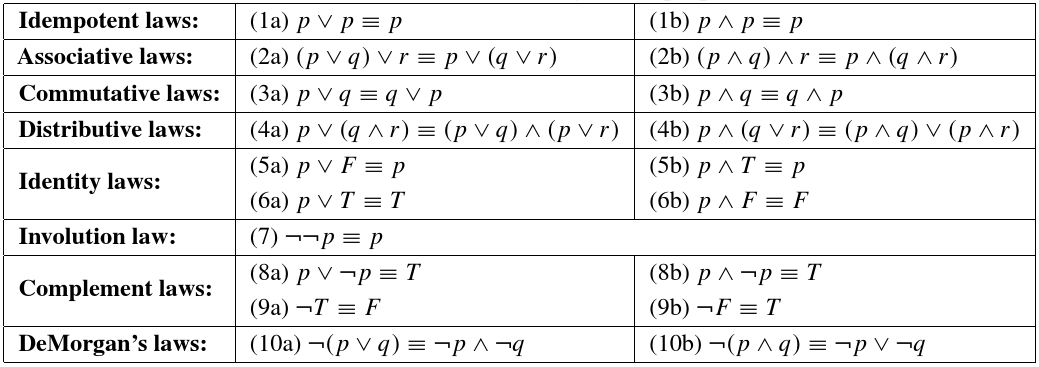
\includegraphics[width=11cm,keepaspectratio=true]{./tabla_4-1.png}
 % tabla_4-1.png: 0x0 pixel, 300dpi, 0.00x0.00 cm, bb=
 \caption{Leyes para el álgebra de proposiciones}
 \label{fig:tabla:4.1}
\end{figure}

\end{frame}

\subsection{Sentencias condicionales y bicondicionales}

\begin{frame}
 Muchas sentencias, particularmente en matem\'aticas, son de la forma \texttt{``si $p$ entonces $q$''}. \pause Tales sentencias son llamdas \emph{condicionales} y son denotadas por 
 $$
 p \imply q.
 $$ 
\end{frame}

\begin{frame}
 El condicional $p \imply q$ es frecuentemente le\'ido como \emph{``$p$ implica $q$''} o \emph{``$p$ s\'olo si $q$''.}
\end{frame}

\begin{frame}
 Otra sentencia com\'un es de la forma \emph{``$p$ si y solo si $q$''.} \pause Tales sentencias son llamadas \emph{bicondicionales} y se denota por 
 $$
 p \iff q.
 $$
\end{frame}

\begin{frame}
 \begin{tdv}[Condicional]
\begin{center}
 \begin{tabular}{|l|l||l|} \hline
$p$ & $q$ & $p \imply q$ \\ \hline
$1$ & $1$ & $1$ \\ \hline
$1$ & $0$ & $0$ \\ \hline
$0$ & $1$ & $1$ \\ \hline
$0$ & $0$ & $1$ \\ \hline
\end{tabular}
\end{center}

 \end{tdv}

\end{frame}

\begin{frame}
 \begin{tdv}[Bicondicional]
\begin{center}
\begin{tabular}{|l|l||l|} \hline
$p$ & $q$ & $p \biconditional q$ \\ \hline
$1$ & $1$ & $1$ \\ \hline
$1$ & $0$ & $0$ \\ \hline
$0$ & $1$ & $0$ \\ \hline
$0$ & $0$ & $1$ \\ \hline
\end{tabular}
\end{center}

 \end{tdv}

\end{frame}

\begin{frame}
 \begin{exmp}
  Demuestre que $$p\imply q \equiv \neg p \vee q.$$
 \end{exmp}

\end{frame}

\begin{frame}
 \begin{evc} Determine cuales de las siguientes sentencias son tautolog\'ias, construyendo las correspondientes tablas de verdad.
  \begin{enumerate}
   \item $\neg\left( p \vee \neg q \right) \imply \neg p$
   \item $p \imply \left( q\imply r \right)$
   \item $\left( p \imply q \right)\imply r$
   \item $\left( p\imply q \right) \imply \left( q\imply p \right)$
   \item $\left( p \wed \left( p \imply q \right) \right) \imply q$
   \item $\left( p \wed q \right) \imply p$
   \item $q \imply \left( \neg p \vee \neg q \right)$
   \item $\left( \left( p\imply q \right) \wed \left( q \imply r \right) \right) \imply \left( p \imply r \right)$
  \end{enumerate}

 \end{evc}

\end{frame}

\subsection{Argumentos}

\begin{frame}
 Un \emph{argumento} es una afirmaci\'on de que un conjunto dado de proposiciones $$P_{1}, P_{2},...,P_{n},$$ llamadas \emph{premisas}, tiene como consecuencia otra proposicion $Q,$ llamada \emph{conclusi\'on.}\pause
 
 En otras palabras, es una sentencia de la forma
 $$
  \left( P_{1} \wed P_{2} \wed...\wed P_{n}\right) \imply Q
  $$
 
 \pause
 
 Tal argumento se denota por $$P_{1}, P_{2},...,P_{n} \yields Q.$$
\end{frame}

\begin{frame}
 La noci\'on de \emph{``argumento l\'ogico''} o \emph{``argumento v\'alido''} se formaliza de la manera siguiente:
 \pause
 
 \begin{defn}
  \label{lip:4.4}
  Un argumento $P_{1}, P_{2},...,P_{n} \yields Q$ se dice que es \emph{v\'alido} si la proposici\'on 
  $$
  \left( P_{1} \wed P_{2} \wed...\wed P_{n}\right) \imply Q
  $$ es una tautolog\'ia.\pause
  
   Si un argumento no es \emph{v\'alido,} diremos que es una \emph{falacia.}
 \end{defn}

\end{frame}

\begin{frame}
 \begin{exmp}
 \label{lip:exmp:4.4}
  \begin{enumerate}
   \item Demuestre que $p, p\imply q \yields q$ es un argumento v\'alido. \pause
   \item Demuestre que $p\imply q, q \yields p$ es una falacia.
   \pause
   \item Demuestre que $p\imply q, \neg q \yields \neg p$ es un argumento v\'alido.
  \end{enumerate}

 \end{exmp}

\end{frame}

\begin{frame}
 \begin{exmp}
  Un principio fundamental del razonamiento l\'ogico nos dice que:
  \begin{center}
   Si $p$ implica $q$ y $q$ implica $r,$ entonces $p$ implica $r.$ 
  \end{center}
\pause

En otras palabras, el siguiente argumento es v\'alido
$$
p\imply,q, q\imply r \yields p \imply r.
$$ \pause
 \end{exmp}

\end{frame}

\begin{frame}
 \begin{figure}
 \centering
 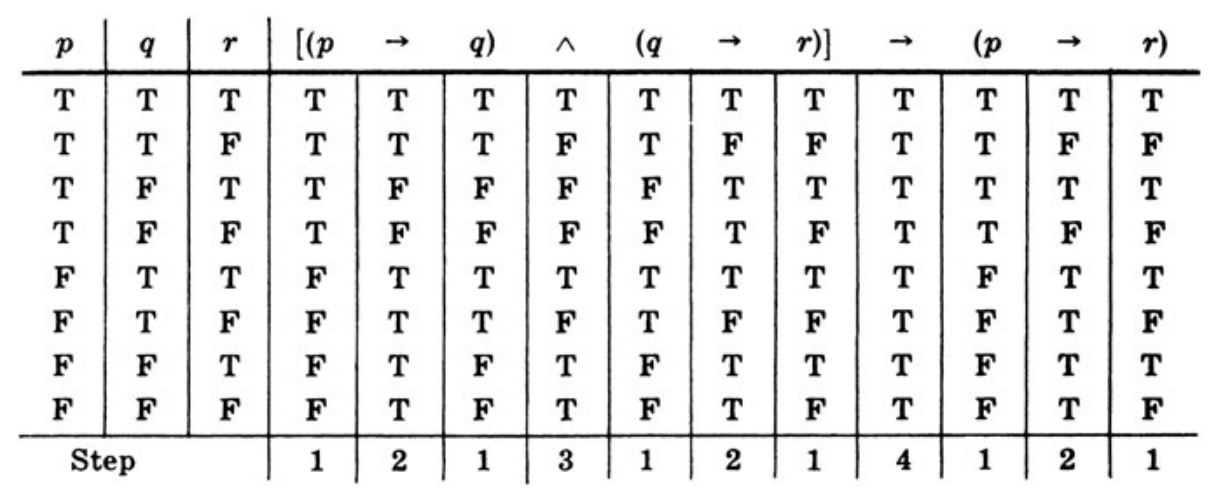
\includegraphics[width=10cm,keepaspectratio=true]{./tabla_silogismo.png}
 % tabla_silogismo.png: 0x0 pixel, 300dpi, 0.00x0.00 cm, bb=
 \label{fig:tabla_silogismo}
\end{figure}

\end{frame}

\begin{frame}
\begin{exmp}
  \begin{center}
\begin{tabular}{l}
Si sube el d\'olar, sube la gasolina.\\
Si sube la gasolina, entonces hay inflaci\'on.\\\hline
$\therefore$ Si sube el d\'olar, entonces hay inflaci\'on.
 \end{tabular}
 \end{center}
\end{exmp}
\end{frame}

\subsection{Funciones proposicionales y Cuantificadores}

\begin{frame}
 Una \emph{funci\'on proposicional} (o \emph{sentencia abierta} o \emph{condici\'on}) definida en un conjunto $A$ es una expresi\'on $p(x)$ que tiene la propiedad de que $p(a)$ es cierta o falsa para cada $a \in A.$
\end{frame}

\begin{frame}
 El conjunto $A$ se conoce como dominio de $p(x),$ y el subconjunto de todos los elementos para los cuales $p(x)$ es cierto se conoce como el \emph{conjunto de verdad} $T_{p}$ de $p(x):$
 \pause
 $$T_{p}=\set{x \mid x\in A, p(x)=\texttt{1}},$$ \pause
 o simplemente 
 $$
 T_{p}=\set{x \mid p(x)}.
 $$
\end{frame}

\begin{frame}
 \begin{exmp}
  \label{lip:exmp:4.7}
  Encuentre el conjunto de verdad para cada funci\'on en el conjunto $\N$ de los enteros positivos:
  \begin{enumerate}
   \item $p(x): x+2>7$ \pause
   \item $p(x): x+5<3$ \pause
   \item $p(x): x+5>1$ 
  \end{enumerate}

 \end{exmp}

\end{frame}

\subsection{Cuantificador universal}

\begin{frame}
 Sea $p(x)$ una funci\'on proposicional definido en un conjunto $A.$ La expresi\'on
 \begin{equation}
 \label{lip:4.1}
   \forall x \in A: p(x)
 \end{equation}

 
 se lee como  \texttt{``para todo $x\in A,$ $p(x)$ es verdadero.''}  \pause
 
 El s\'imbolo $\forall$ (\texttt{``para todo''}) se llama cuantificador universal.
\end{frame}


\begin{frame}
 Mientras que $p(x)$ es una sentencia abierta (su valor de verdad depende de cada $x\in A$), la afirmaci\'on 
 $$\forall x\in A: p(x)$$ es verdadera si y solo si $p(x)$ se cumple para todo $x\in A.$  
\end{frame}

\begin{frame}
 Por otro lado, si existe alg\'un $x\in A$ tal que $p(x)$ es falso, entonces $$\forall x\in A: p(x)$$ es falso.
\end{frame}

\begin{frame}
 \begin{exmp}
  \label{lip:exmp:4.8}
  Verifique el valor de verdad de las siguientes afirmaciones:
  \begin{enumerate}
   \item $\forall n \in \N: n+4>3.$ \pause
   \item $\forall n \in \N: n+2>8.$
  \end{enumerate}

 \end{exmp}

\end{frame}

\subsection{Cuantificador existencial}

\begin{frame}
 Sea $p(x)$ una funci\'on proposicional definido en un conjunto $A.$ La expresi\'on
 \begin{equation}
 \label{lip:4.3}
   \exists x \in A: p(x)
 \end{equation} 
 se lee como  \texttt{``existe $x\in A,$ tal que $p(x)$ es verdadero.''}  \pause
 
 El s\'imbolo $\exists$ (\texttt{``existe...''}) se llama cuantificador existencial.
\end{frame}


\begin{frame}
 Mientras que $p(x)$ es una sentencia abierta (su valor de verdad depende de cada $x\in A$), la afirmaci\'on 
 $$\exists x\in A: p(x)$$ es verdadera si y solo si $p(x)$ se cumple alg\'un $x\in A.$  
\end{frame}

\begin{frame}
 Por otro lado, si para todo $x\in A,$ $p(x)$ es falso, entonces $$\exists x\in A: p(x)$$ es falso.
\end{frame}

\begin{frame}
 Verifique el valor de verdad de las siguientes afirmaciones:
 \begin{enumerate}
  \item $\exists n  \in \N: n+4<7;$ \pause
  \item $\exists n \in \N: n+6<4.$
 \end{enumerate}

\end{frame}

\subsection{Negaci\'on de Sentencias Cuantificadas}


\begin{frame}
 Considere la afirmaci\'on:
 \begin{center}
  \emph{Todos los estudiantes de ingenier\'ia saben programar.}
 \end{center}
?`C\'omo podemos negar esta afirmaci\'on?
\pause

\begin{center}
 \emph{Al menos un estudiante de ingenier\'ia no sabe programar.}
\end{center} 
\end{frame}

\begin{frame}
 De manera simb\'olica, si $M$ de ntoa el conjunto de estudiantes de ingenier\'ia, la negaci\'on anterior se puede escribir como
\begin{align*}
  \neg\left( \forall x\in M: \texttt{x sabe programar} \right)\\ \equiv \exists x\in M: \texttt{x no sabe programar.}
\end{align*}

\end{frame}

\begin{frame}
 Si en el ejercicio anterior definimos $$p(x):\texttt{x sabe programar},$$ entonces podemos reescribir la equivalencia anterior como
 \begin{align*}
  \neg\left( \forall x\in M: p(x) \right)\\ \equiv \exists x\in M: \neg p(x).
\end{align*}
\end{frame}

\begin{frame}
 De manera similar
 \begin{center}
  \emph{No hay estudiante de ingenier\'ia que sepa programar}
 \end{center}
 se puede reescribir como
 \begin{center}
  \emph{Cada uno de los estudiantes de ingenier\'ia no saben programar.}
 \end{center}


\end{frame}

\begin{frame}
 De manera simb\'olica, podemos reescribir
  \begin{align*}
  \neg\left( \exists x\in M: p(x) \right)\\ \equiv \forall x\in M: \neg p(x).
\end{align*}
\end{frame}

\begin{frame}
 \begin{thm}[DeMorgan]
  \begin{align}
  \label{lip:thm:4.4}
   \neg\left( \forall x\in M: p(x) \right)& \equiv \exists x\in M: \neg p(x)\\
   \label{lip:thm:4.5}
   \neg\left( \exists x\in M: p(x) \right)& \equiv \forall x\in M: \neg p(x).
  \end{align}

 \end{thm}

\end{frame}

\begin{frame}
 \begin{exmp}
  \label{lip:exmp:4.10.a}
  La negaci\'on de la siguiente afirmaci\'on
  \begin{center}
   \emph{Para todo entero positivo $n,$ tenemos que $n+2>8$}
  \end{center}
es 
\begin{center}
 \emph{Existe un entero positivo $n$ tal que $n+2 \leq 8.$}
\end{center}

 \end{exmp}

\end{frame}

\begin{frame}
 \begin{exmp}
  \label{lip:exmp:4.10.b}
  La negaci\'on de la siguiente afirmaci\'on
  \begin{center}
   \emph{Existe una persona viva con 150 a\~nos o m\'as.}
  \end{center}
 es 
 \begin{center}
  \emph{Toda persona viva tiene menos de 150 a\~nos.}
 \end{center}

 \end{exmp}

\end{frame}

\begin{frame}
 \begin{rem}
  Para negar una afirmaci\'on del tipo $$\forall x \in A: p(x)$$ s\'olo necesitamos encontrar un elemento $x_{0}\in A$ tal que $p(x)$ sea \emph{falso.}
  \pause
  
  A un elemento $x_{0}$ as\'i se le conoce como \emph{contraejemeplo.}
 \end{rem}

\end{frame}

\begin{frame}
 \begin{exmp}
 \label{lip:4.11}
  \begin{enumerate}[(a)]
   \item 
  Un contraejemplo para $\forall x \in \R: \abs{x}\neq 0$ es $x=0.$  \pause
   \item 
  Un contraejemplo para $\forall x \in \R: x^{2}\geq x$ es $x=\frac{1}{2}.$  \pause
   \item 
  Sin embargo, $\forall x \in \N: : x^{2}\leq x$ es siempre cierto.
  \end{enumerate}

 \end{exmp}

\end{frame}

\subsection{Ejercicios Resueltos}

\subsubsection{Proposiones y Tablas de Verdad}

\begin{frame}
 \begin{solved}
  Sea $p:\texttt{``Hace fr\'io''}$ y $q:\texttt{``Est\'a lloviendo''.}$ Proponga un enunciado verbal simple que describa cada una de las siguientes proposiciones:
  \begin{enumerate}
   \item $\neg p;$
   \item $p \wed q;$
   \item $p \vee q;$
   \item $q \vee \neg p.$
  \end{enumerate}

 \end{solved}

\end{frame}

\begin{frame}
 \begin{solved}
  Encuentre la tabla de verdad de $\neg p \wed q.$
 \end{solved}

\end{frame}

\begin{frame}
 \begin{solved}
  Demuestre que la propisici\'on 
  $$
  p \vee \neg \left( p\wed q \right)
  $$ es una tautolog\'ia.
 \end{solved}

\end{frame}

\begin{frame}
 \begin{solved}
  Muestre que las proposiciones $\neg\left( p \wed q \right)$ y $\neg p \vee \neg q$ son l\'ogicamente equivalentes.
 \end{solved}

\end{frame}

\begin{frame}
 \begin{solved}
  Use las leyes en la tabla \ref{fig:tabla:4.1} para mostrar que 
  $$
  \neg \left( p \wed q \right) \vee \left( \neg p \wed  q \right) \equiv \neg p
  $$
 \end{solved}

\end{frame}

\subsubsection{Sentencias condicionales}

\begin{frame}
 \begin{solved}
  \label{lip:sol:4.6}
  Reescriba los siguientes enunciados sin usar el condicional:
  \begin{enumerate}
   \item Si hace fr\'io, el usa sombrero. \pause
   \item Si la productividad se incrementa, entonces el salario aumenta.
  \end{enumerate}

 \end{solved}

\end{frame}

\begin{frame}
 \begin{solved}
  \label{lip:sol:4.7}
  Considere la proposici\'on condicional $p \imply q.$ La proposiones 
  \begin{center}
  ${\color{red}q \imply p,} {\color{blue}\, \neg p \imply \neg q,} \, {\color{green}\neg q \imply \neg p}$
  \end{center}
son llamadas {\color{red} conversa,} {\color{blue}inversa} y {\color{green} contrapositiva}, respectivamente.
\pause

?`Cu\'ales de estas proposiciones son l\'ogicamente equivalente s a $p\imply q$?
 \end{solved}

\end{frame}

\begin{frame}
 \begin{solved}
  Determine la contrapositiva de cada enunciado:
  \begin{enumerate}
   \item Si Erik es poeta, entonces es pobre. \pause
   \item Solo si Marcos estudia, pasar\'a el examen. 
  \end{enumerate}

 \end{solved}

\end{frame}

\begin{frame}
 \begin{solved}
  Escriba la negaci\'on de cada enunciado, tan simple como sea posible:
  \begin{enumerate}
   \item Si ella trabaja, ganar\'a dinero. \pause
   \item El nada si y solo si el agua est\'a tibia. \pause
   \item Si neva, entonce no manejar\'e.
  \end{enumerate}

 \end{solved}

\end{frame}

\subsubsection{Argumentos}

\begin{frame}
 \begin{solved}
  Muestre que el siguiente argumento es una falacia:
 $$
 p\imply q, \neg p \yields \neg q.
 $$
 \end{solved}

\end{frame}

\begin{frame}
 \begin{solved}
  Muestre que el siguiente argumento es v\'alido:
 $$
 p\imply q, \neg q \yields \neg p.
 $$
 \end{solved}

\end{frame}

\begin{frame}
\begin{solved}
  Muestre que el siguiente argumentos siempre es v\'alido:
 $$
 p \imply \neg q, r \imply q, r \yields \neg p.
 $$
\end{solved}

\end{frame}

\begin{frame}
 \begin{solved}
  Determine la validez del siguiente argumento:
  \begin{center}
\begin{tabular}{l}
Si $7$ es menor que $4$, entonces $7$ no es n\'umero primo\\
$7$ no es menor que $4$\\\hline
$7$ no es n\'umero primo.
  \end{tabular}
  \end{center}

 \end{solved}

\end{frame}

\begin{frame}
 \begin{solved}
  Determine la validez del siguiente argumento:
  \begin{center}
\begin{tabular}{l}
Si dos lados de un tri\'angulo son iguales, entonces los respectivos \'angulos opuestos son iguales\\
Dos lados de un tri\'angulo no son iguales\\\hline
Los respectivos \'angulos opuestos no son iguales.
  \end{tabular}
  \end{center}

 \end{solved}

\end{frame}

\subsubsection{Cuantificadores y Funciones Proposicionales}

\begin{frame}
 \begin{solved}
  Sea $A=\set{1,2,3,4,5}.$ Determine el valor de verdad de cada uno de los siguientes enunciados:
  \begin{enumerate}
   \item $\exists x \in A: x+3=10;$ \pause
   \item $\forall x \in A: x+3<10;$ \pause
   \item $\exists x \in A: x+3<5;$ \pause
   \item $\forall x \in A: x+3 \leq 7.$
  \end{enumerate}

 \end{solved}

\end{frame}

\begin{frame}
  \begin{solved}
    Determine el valor de verdad de cada uno de las siguientes afirmaciones donde $U=\set{1,2,3}$ es el conjunto \emph{``universo''} (de referencia):
 \begin{enumerate}
  \item $\exists x \forall y: x^{2}< y+1;$ \pause
  \item $\forall x \exists y: x^{2}+y^{2}<12;$ \pause
  \item $\forall x \forall y: x^{2}+y^{3}<12.$
 \end{enumerate}

  \end{solved}

\end{frame}

\begin{frame}
 \begin{solved}
  Encuentre la negaci\'on de cada una de las siguientes afirmaciones:
  \begin{enumerate}
   \item $\exists x \forall y: p(x,y);$ \pause
   \item $\forall x \forall y: p(x,y);$ \pause
   \item $\exists x \exists y \forall z: p(x,y,z).$
  \end{enumerate}

 \end{solved}

\end{frame}

\begin{frame}
 \begin{solved}
  Sea $$p(x): x+2>5.$$ Indique cuando $p(x)$ es una funci\'on proposicional o no en cada uno de los siguientes conjuntos: 
  \begin{enumerate}
   \item $\N$ \pause
   \item $\Z^{-}=\set{-1,-2,-3,...}$ \pause
   \item $\mathbb{C}$
  \end{enumerate}

 \end{solved}

\end{frame}

\begin{frame}
	\begin{evc}
	Niegue cada uno de las siguientes afirmaciones:
	\begin{enumerate}
		\item Todos los estudiantes viven en los dormitorios.
		\item A todos los estudiantes de ingeniería le gusta el futbol.
		\item Algunos estudiantes tienen 25 años o más.
	\end{enumerate}
	\end{evc}
\end{frame}

\begin{frame}
 \frametitle{Bibliograf\'ia}
 Las notas de esta secci\'on est\'an basadas en el cap\'itulo 4 \texttt{``Logic and Propositional Calculus''} del libro
 \begin{center}
  \texttt{Lipschutz, S. and Lipson, M.;\textbf{ Schaum's Outline of Discrete Mathematics;} McGraw-Hill, 3th Edition.}
 \end{center}

\end{frame}

\end{document}